\documentclass{memoria}


\begin{document}

\portada{Informe Entrega 2: Diseño Arquitectural}{Gerson Aguirre Pavez\\Max Chacón Villanueva\\Daniel Gacitúa Vásquez\\Elías González Marincovic\\Nicolás Rozas Sepúlveda}{\textbf{Profesores:}\\Mauricio Marín Caihuán\\Rodrigo Vásquez Fernández\\\textbf{Ayudante:\\}José Orellana}{\today}


\indices

\capitulonn{INTRODUCCIÓN.}

En esta entrega se presenta la etapa de diseño arquitectural de la aplicación \textbf{\textsl{BitPhoto}}, réplica de \textsl{Flickr}.  El objetivo de esta etapa es construir la arquitectura básica para el funcionamiento de la aplicación, definiendo los diversos componentes del sistema acordes a la solución necesitada. Para especificar de manera más detallada la arquitectura del sistema se utilizará el modelo 4 + 1 vistas, el cual nos permite definir en cada una de sus vistas una parte esencial de la arquitectura del sistema, y de manera conjunta ofrecer una visión específica en diversos niveles, desde saber cuáles son los componentes involucrados, dónde se despliegan, y de qué manera interactúan entre ellos para cumplir con los requerimientos especificados en la entrega anterior, correspondiente a la ingeniería de requerimientos.
 
En este informe se presenta inicialmente un marco teórico utilizado para contextualizar el contenido y al mismo tiempo hacer referencia conceptual a éste. Luego continuando con el cumplimiento de los objetivos, se presenta el modelo 4 + 1 vistas, que servirá para explicar todos los elementos anteriormente mencionados. Para desarrollar este modelo, en primera instancia se trata la \textsl{Vista Lógica}, y es en esta parte donde se detallan los módulos del sistema que entregan la funcionalidad característica del mismo, asemejándose al diagrama de clases presentado con anterioridad. Continuando con las vistas, se presenta la \textsl{Vista de Proceso} donde se muestran los aspectos de concurrencia y sincronización correcta del sistema para el óptimo funcionamiento de la aplicación. Luego, la \textsl{Vista Física} permite observar el \textsl{mapeo} del software y analizar de qué manera se distribuye y posteriormente, en la \textsl{Vista de Desarrollo} se muestra la forma en que se despliega el software en el ambiente de desarrollo. 

Después de las vistas, se presentan eventuales escenarios, en los cuales se aprecia la forma en que se comporta el sistema y de qué manera interactúan los módulos y componentes de éste para realizar determinadas acciones asociadas a los diferentes casos de uso. Luego, para dar una visión globalizada de la arquitectura del sistema, se utiliza el \textsl{framework} conceptual de \textsl{SunTone}, que se representa en forma de cubo, detallando de esta forma la calidad del sistema, los niveles de lógica y de servicios de infraestructura en cada una de sus caras. Además, con el fin de comprender de mejor manera la arquitectura del sistema, se señalan los diferentes tipos de \textsl{frameworks} tecnológicos y conceptuales utilizados, definiendo los patrones de diseños que se usarán y los problemas que estos solucionan. Por último, luego de haber especificado el diseño arquitectural, se presenta en detalle cuáles serán las tecnologías utilizadas por el sistema, describiendo cada una de éstas, señalando la versiones que se utilizarán y definiendo cuál es el problema que resuelven o la funcionalidad que aportan. 

Para finalizar el informe, se entregará un detalle sobre la planificación y organización de este \textsl{sprint}, detallando las tareas definidas y la estimación de tiempo para cada una de éstas, para luego mostrar los gráficos \textsl{Burn Down} y \textsl{Burn Up}, los que señalarán de qué manera se desarrolló el trabajo entregado con el paso de los días para hacer el análisis pertinente referente al desarrollo de la entrega, identificando las principales dificultades y los cambios realizados con respecto al \textsl{sprint} anterior, entre otras cosas. 

En resumen, se puede establecer que el objetivo de este informe es definir la arquitectura del sistema, identificando cuales deben ser los componentes del mismo, con el fin de satisfacer los requisitos especificados en la entrega pasada. También se busca definir de qué manera se distribuirán estos componentes en el sistema y en qué máquinas de hardware se van a desplegar y todo este conocimiento deberá servir como base para el desarrollo de la siguiente entrega (correspondiente al diseño detallado) donde se especificará la arquitectura pero llevada a la tecnología utilizada (especificada en este documento) y a las características propias de éstas.

%-------------------------------------------------------------------------------------
\capitulo{MARCO TEÓRICO.}

\seccion{MODELO 4+1 VISTAS.}

Este modelo, es una forma de representar una arquitectura de aplicación, el que requiere múltiples vistas para su entendimiento. Este recurso permite abordar los intereses de los distintos \textsl{stakeholders} de la arquitectura por separado: usuarios finales, desarrolladores, ingenieros de sistemas, administradores de proyecto, etc. Y de esta manera poder manejar los requisitos funcionales y no funcionales separadamente.

Las vistas definidas en este modelo, son las siguientes:

\begin{itemize}
\item \textbf{Vista Lógica}: describe el modelo de objetos del diseño cuando se utiliza un método de diseño orientado a objetos. Para modelar una aplicación que esté orientada a los datos, se puede usar un enfoque alternativo para desarrollar algún otro tipo de vista lógica, tal como diagramas de entidad-relación.
\item \textbf{Vista de Procesos}: se enfoca en la descripción de los aspectos de concurrencia y sincronización del diseño. La arquitectura de procesos toma en cuenta algunos requisitos no funcionales tales como la performance y la disponibilidad. Se centra en asuntos de concurrencia y distribución, integridad del sistema y de tolerancia a fallas. La vista de procesos también específica en cual hilo de control se ejecuta efectivamente una operación de una clase identificada en la vista lógica.
\item \textbf{Vista Física}: se encarga de describir el mapeo del software en el hardware y refleja los aspectos de distribución. La arquitectura física toma en cuenta primeramente los requisitos no funcionales del sistema tales como la disponibilidad, confiabilidad (con respecto a la tolerancia a fallas), performance (throughput), y escalabilidad. El software se ejecuta sobre una red de computadoras o sobre nodos de procesamiento (o en algunos casos tan solo nodos). Los variados elementos identificados –tales como redes, procesos, tareas y objetos– requieren ser mapeados sobre los variados nodos existentes. Se espera que se puedan utilizar diferentes configuraciones, algunas para desarrollo y pruebas, y otras para emplazar el sistema en varios sitios para distintos usuarios.
\item \textbf{Vista de Desarrollo}: escribe la organización estática del software en su ambiente de desarrollo. La vista de desarrollo se centra principalmente en la organización real de los módulos que interactúan en el sistema, en el ambiente de desarrollo del software. El software se empaqueta en partes pequeñas –como bibliotecas de programas o subsistemas– que pueden ser desarrollados por uno o un grupo pequeño de desarrolladores. Los subsistemas se organizan en una jerarquía de capas, cada una de las cuales brinda una interfaz estrecha y bien definida hacia las capas superiores.
\item \textbf{Escenarios (+1)}: corresponde a la ilustración de un conjunto reducido de casos de uso o escenarios, los cuales constituyen la quinta vista (en el caso concreto, la vista \textsl{+1}. La arquitectura evoluciona parcialmente a partir de estos escenarios.
\end{itemize}

\figura{Modelo 4+1 vistas.}{
	\centering
	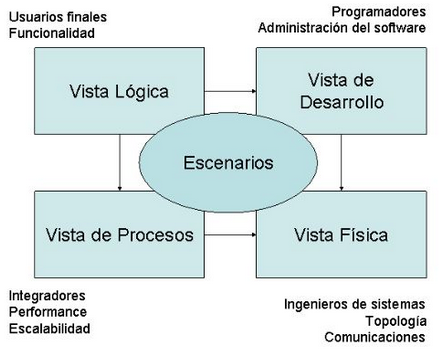
\includegraphics[width=14cm]{modelo4+1vistas.png}
}

En la figura 1-1 se puede apreciar una representación del modelo 4+1 vistas, mostrando una relación entre las diferentes vistas y los actores y/o elementos que participan en cada una de ellas.

\seccion{MODELO 3-DIMENSIONAL SUNTONE.}

Este modelo es un framework que permite conocer y visualizar de manera global la arquitectura del sistema. Está compuesto por tres dimensiones que se detallan a continuación:

\begin{itemize}
\item \textbf{DIMENSIÓN: NIVELES LOGICOS.}

El estándar de arquitectura para aplicaciones distribuidas, separa la lógica de la aplicación en un número determinado de niveles. Estos niveles representan una organización lógica y física de los componentes en una cadena ordenada entre los proveedores de servicios y consumidores. Los componentes dentro de un nivel suelen consumir los servicios prestados por otros componentes distintos en un nivel de proveedor adyacente, y a su vez proporcionan servicios a uno o más componentes en otro nivel de consumo adyacente.
\newpage

\item \textbf{DIMENSIÓN: NIVELES DE SERVICIO DE INFRAESTRUCTURA.}

Los componentes de software que interactúan entre sí, provenientes de aplicaciones empresariales distribuidas, requieren un conjunto subyacente de servicios e  infraestructura que permite a los componentes distribuidos comunicarse entre sí, coordinar su trabajo, implementar un acceso seguro, entre otras funciones. Este conjunto de servicios distribuidos constituye una infraestructura sobre la que se distribuyen los componentes que se pueden construir.

\item \textbf{DIMENSIÓN: CALIDAD DE SERVICIO.}

Las dos dimensiones arquitectónicas anteriores (capas lógicas y niveles de servicio de infraestructura), definen en gran medida los aspectos lógicos de la arquitectura. Sin embargo, una dimensión igualmente importante de cualquier solución implementada, es la capacidad de cumplir con requisitos de calidad de servicio. Como los servicios de Internet y de comercio electrónico se han vuelto más críticos para las operaciones de negocio, tanto el rendimiento como la disponibilidad, seguridad, escalabilidad y capacidad de servicio, se ha convertido en un requisito clave de gran escala para arquitecturas de despliegue de alto rendimiento. En otras palabras, el cumplimiento de los requerimientos del negocio en relación con una serie de cualidades importantes de servicios, se ha convertido en una dimensión importante de la arquitectura. 
\end{itemize}

Las tres dimensiones arquitectónicas discutidas por separado en los apartados anteriores, en su conjunto proporcionan un marco para entender el papel de cualquier aplicación o componente de infraestructura dentro de un diseño arquitectónico. Básicamente, componentes distribuidos en cada nivel lógico de una arquitectura de despliegue (la primera dimensión) necesitan ser apoyados por los servicios de infraestructura adecuados (la segunda dimensión). Cada componente dentro de esa matriz de dos dimensiones deben implementarse de acuerdo a los requisitos propuestos con el fin de mejorar la  calidad del servicio (la tercera dimensión).

Las tres dimensiones anteriormente detalladas, se pueden representar en un cubo, ubicando cada una de ellas en una cara del mismo, tal como lo muestra la figura 1-2.

\newpage
\figura{Modelo 3-Dimensional SunTone.}{
	\centering
	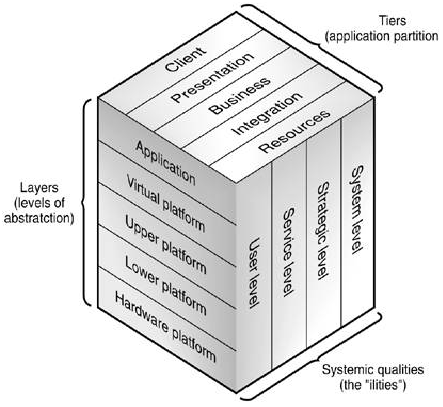
\includegraphics[width=13cm]{cuboSunTone.png}
}

\seccion{PATRONES DE DISEÑO.}

Los patrones de diseño son el esqueleto de las soluciones a problemas comunes en el desarrollo de software. En otras palabras, brindan una solución ya probada y documentada a problemas de desarrollo de software que están sujetos a contextos similares. Se debe tener presente los siguientes elementos de un patrón: su nombre, el problema (cuando aplicar un patrón), la solución (descripción abstracta del problema) y las consecuencias (costos y beneficios).

Los patrones de diseño se pueden clasificar en tres tipos distintos:

\begin{itemize}
\item \textbf{Patrones Creacionales}: la función de estos patrones es la inicialización y configuración de distintos objetos, en otras palabras, se encargan de la creación de objetos para su posterior utilización.
\item \textbf{Patrones Estructurales}: se encargan de separar la interfaz de la implementación. Se ocupan de cómo se agrupan las clases y objetos, para formar estructuras más grandes.
\item \textbf{Patrones de Comportamiento}: como el nombre lo indica, estos patrones se encargan de describir la comunicación que existe entre los objetos o las clases mas que describir éstos como tal.
\end{itemize}

\subseccion{MODELO VISTA-CONTROLADOR (MVC).}

La mayoría de las arquitecturas de aplicaciones web se basan en este patrón o variaciones de éste, y a su vez la plataforma a utilizar (Java EE) trabaja bajo esta lógica. El modelo MVC, se caracteriza por ser un patrón que separa la lógica de negocio de la interfaz de usuario, facilitando así la evolución por separado de ambas capas.

\begin{itemize}
\item La capa \textbf{modelo} representa la realidad.
\item La capa \textbf{controlador}, conoce los métodos y atributos del modelo. Recibe y realiza lo que el usuario quiere hacer, en otras palabras, gestiona la funcionalidad del sistema.
\item La capa \textbf{vista} muestra un aspecto del modelo y es utilizada por la capa modelo para lograr la interacción con el usuario. (No existe comunicación directa entre la capa modelo y la capa vista)
\end{itemize}


\subseccion{PATRONES DE DISEÑO EN JavaEE}

La arquitectura de J2EE se divide cuatro capas principalmente: Presentación – Negocios – Integración – Recursos (Datos). Dentro de estas capas se presentan distintos patrones utilizados (a excepcion de la capa de recursos) detallados a continuación:

\begin{itemize}
\item \textbf{CAPA DE PRESENTACIÓN.}

\begin{itemize}
\item \textbf{\textsl{Decorating Filter /Intercepting Filter}}: el mecanismo de manejo de peticiones de la capa de presentación recibe muchos tipos diferentes de peticiones, cada uno de los cuales requiere varios tipos de procesamiento. Algunas peticiones  simplemente requieren su reenvío al componente manejador apropiado, mientras que otras peticiones deben ser modificadas, auditadas, o descomprimidas antes de su procesamiento posterior.

\item \textbf{\textsl{Front Controller/Front Component}}: el mecanismo de manejo de peticiones de la capa de presentación debe controlar y coordinar el procesamiento de todos los usuarios a través de varias peticiones. Dichos mecanismos de control se  pueden manejar de una forma centralizada o descentralizada. 
 
Es un objeto que acepta todos los requerimientos de un cliente y los direcciona a manejadores apropiados. El patrón \textsl{Front Controller} podría dividir la funcionalidad en 2 diferentes objetos: el \textsl{Front Controller} y el \textsl{Dispatcher}. En ese caso, El \textsl{Front Controller} acepta todos los requerimientos de un cliente y realiza la autenticación. El \textsl{Dispatcher}, por su parte, direcciona los requerimientos a manejadores apropiados.

\item \textbf{\textsl{View Helper}}: el sistema crea el contenido de la presentación, lo que requiere el procesamiento de datos de negocio dinámicos. Normalmente es un objeto \textsl{helper} que encapsula la lógica de acceso a datos en beneficio de los componentes de la presentación. Por ejemplo, los \textsl{JavaBeans} pueden ser usados como patrón \textsl{View Helper} para las páginas JSP.

\item \textbf{\textsl{Composite view}}: las páginas Web sofisticadas presentan contenido de varias fuentes de datos, utilizando varias subvistas que completan una sola página. Además, varios individuos con diferentes habilidades contribuyen al desarrollo y mantenimiento de esas páginas Web. Se puede ver como un objeto vista que está compuesto de otros objetos vista, por ejemplo, una página JSP que incluye otras páginas JSP y HTML usando la directiva \textsl{include} o el \textsl{action include} es un patrón \textsl{Composite View}.

\item \textbf{\textsl{Service to Worker}}: el sistema controla el flujo de ejecución y accede a los datos de negocio, desde los que crea el contenido de la presentación.
Es como el patrón de diseño MVC con el Controlador actuando como \textsl{Front Controller} pero con un detalle importante: aquí el \textsl{Dispatcher} (el cual es parte del \textsl{Front Controller}) usa \textsl{View Helpers} a gran escala y ayuda en el manejo de la vista.

\item \textbf{\textsl{Dispatcher View}}: cumple con la misma función que el patrón \textsl{Service to Work} pero contrario a éste, aquí el \textsl{Dispatcher} no usa \textsl{View Helpers} y realiza muy poco trabajo en el manejo de la vista. El manejo de la vista es manejado por los mismos componentes de la Vista.
\end{itemize}

\item \textbf{CAPA DE NEGOCIOS.}

\begin{itemize}
\item \textbf{\textsl{Business Delegate/ Bussines Object}}: un sistema multi-capa distribuido requiere invocación remota de métodos para enviar y recibir datos entre las capas. Los clientes están expuestos a la complejidad de tratar con componentes distribuidos. Se puede ver como un objeto que reside en la capa de presentación y en beneficio de los otros componentes de la capa de presentación llama a métodos remotos en los objetos de la capa de negocios.

\item \textbf{\textsl{Value Object/ Data Transfer Object/ Replicate Object}}: cuando las aplicaciones cliente necesitan intercambiar datos con \textsl{Beans Enterprise} se puede crear un objeto serializable para la transferencia de datos sobre la red.

\item \textbf{\textsl{Session Facade/Session Entity Facade/Distributed Facade}}: los \textsl{Beans Enterprise} encapsulan lógica y datos de negocio y exponen sus interfaces, y con ellos la complejidad de los servicios  distribuidos, a la capa de cliente. El uso de un bean de sesion como una fachada (\textsl{facade}) para encapsular la complejidad de las interacciones entre los objetos de negocio y participantes en un flujo de trabajo. El \textsl{Session Facade} maneja los objetos de negocio y proporciona un servicio de acceso uniforme a los clientes.

\item \textbf{\textsl{Aggregate Entity/Composite Entity}}: puede ser visto como un bean entidad que es construido o es agregado a otros beans de entidad. Los beans de entidad no se han pensado para representar todos los objetos persistentes del modelo y son mejores  para objetos de negocio persistentes genéricos.

\item \textbf{\textsl{Value Object Assembler/Transfer Object Assambler}}: en una aplicación de la plataforma JavaEE, los componentes de negocio del lado del servidor se implementan utilizando \textsl{beans} de sesión, \textsl{beans} de entidad, DAOs, etc. Los clientes de la aplicación necesitan acceder a datos que frecuentemente se componen de múltiples objetos. Un objeto que reside en la capa de negocios y crea \textsl{Value Objects} cuando es requerido.

\item \textbf{\textsl{Value List Handler/Page-by-Page Iterator/Paged List}}: el cliente le pide al servicio una lista de ítems para su presentación. El número de ítems de la lista no se conoce y puede ser muy grande en muchas circunstancias. Se puede ver como un objeto que maneja la ejecución de consultas SQL, caché y procesamiento del resultado. Usualmente implementado como \textsl{beans} de sesión.

\item \textbf{\textsl{Service Locator}}: la búsqueda y creación de servicios implican interfaces complejas y operaciones de red. Consiste en utilizar un objeto \textsl{Service Locator} para abstraer toda la utilización JNDI y para ocultar la complejidad de la creación del contexto inicial, de búsqueda de objetos home EJB y recreación de objetos EJB. Varios clientes pueden reutilizar el objeto \textsl{Service Locator} para reducir la complejidad del código, proporcionando un punto de control.
\end{itemize}

\item \textbf{CAPA DE INTEGRACIÓN.}

\begin{itemize}
\item \textbf{\textsl{Data Access Object/Service Activator}}: el acceso a los datos varía dependiendo de la fuente de los datos. El acceso al almacenamiento persistente, como una base de datos, varía en gran medida dependiendo del tipo de almacenamiento
(bases de datos relacionales, bases de datos orientadas a objetos, ficheros planos, entre otros) y de la implementación del vendedor. Consiste en utilizar un objeto de acceso a datos para abstraer y encapsular todos los accesos a la fuente de datos. El DAO maneja la conexión con la fuente de datos para obtener y almacenar datos. 

\item \textbf{\textsl{Service Activator}}: los \textsl{beans enterprise} y otros servicios de negocio, necesitan en ocasiones una forma de activarse asíncronamente.
Se utiliza para recibir peticiones y mensajes asíncronos de los clientes. Cuando se recibe un mensaje, el \textsl{Service Activator} localiza e invoca a los métodos de los componentes de negocio necesarios para cumplir la petición de forma asíncrona.
\end{itemize}

\end{itemize} 

%-------------------------------------------------------------------------------------
\capitulo{MODELO 4+1 VISTAS.}

Como se mencionó en el marco teórico (ver sección 1.1), el modelo 4+1 vistas se basa en 4 vistas principales además de los escenarios que se presenten. Las vistas desarrolladas, correspondientes a la aplicación, se presentan a continuación.

\seccion{VISTA LÓGICA.}

\figura{Vista Lógica de aplicación \textsl{BitPhoto}.}{
	\centering
	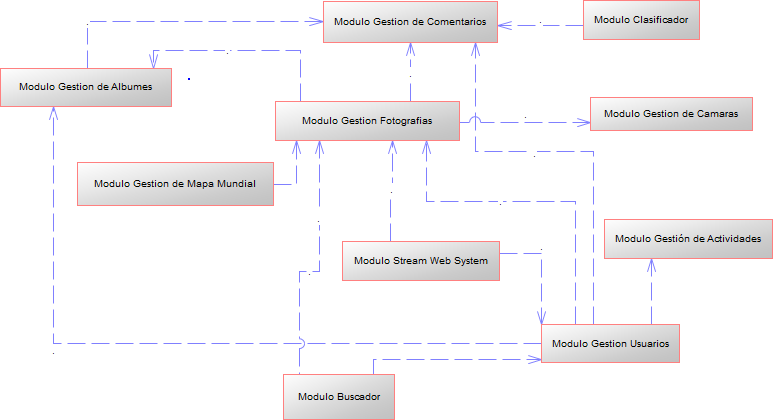
\includegraphics[width=17cm, height=12cm]{vistaLogica.png}
}

En esta ocasión se tienen diez módulos distintos para representar las funcionalidades que va a poseer el sistema. A continuación se procede a describir que realiza cada uno de éstos.

\begin{itemize}
\item \textbf{Módulo Gestión Fotográfica}: en este módulo se representan las funcionalidades que tienen relación a la carga de fotografías por parte del usuario, además de las funcionalidades de realizar las respectivas descripciones a éstas, incluyendo así la vista en el sistema de las fotografías y sus movimientos en la base de datos, es decir, la creación, actualización, eliminación y las consultas correspondientes que se pueden realizar con respecto a éstas.

\item \textbf{Módulo Gestión de Comentarios}: acá se ven las funcionalidades de la realización de un comentario, ya sea en una fotografía que ha sido cargada por el mismo usuario o por algún otro usuario al cual se está siguiendo, además de marcar los favoritos que el usuario desea realizar, así como también el manejo de los \textsl{tags} que pueden estar contenidos en los comentarios.

\item \textbf{Módulo Clasificador}: en este módulo se representan las funcionalidades con respecto la tecnología WEKA, donde se desea clasificar cada uno de los comentarios con una evaluación, éstas pueden ser positivo, negativo o neutral según corresponda.

\item \textbf{Módulo Gestión de Álbumes}: acá se ven las funcionalidades que pertenecen a los álbumes, es decir, seleccionar una fotografía de portada del álbum o agregar un nombre a éste, además de agregar una descripción correspondiente si el usuario lo desea. En resumen, se representa la funcionalidad de la visualización de los álbumes en la vista correspondiente a estos.

\item \textbf{Módulo Gestión del Mapa Mundial}: en este módulo se representan las funcionalidades con respecto al mapa mundial, en el que se podrá realizar una búsqueda de fotografías populares por medio de una ubicación geoespacial.

\item \textbf{Módulo Gestión de Cámaras}: se representan las funcionalidades de asociación de una cámara a una fotografía, es decir, se mostrarán las características de una cámara en las fotografías que han sido tomadas con ésta.

\item \textbf{Módulo Gestión de Actividades}: en este módulo se representa el manejo de los movimientos que realizan los seguidores y el usuario como tal, de manera que el usuario pueda visualizar los últimos eventos realizados por él y sus seguidores.

\item \textbf{Módulo Gestión de Usuarios}: se representan las funcionalidades que se pueden realizar en consideración al usuario, éstas contemplan el manejo de un perfil, donde él podrá realizar algunos cambios en su información personal.

\item \textbf{Módulo Buscador}: en este módulo se representa la función de realizar una búsqueda de usuarios y fotografías en el sistema. Un usuario puede buscar ciertas fotografías que tengan asociadas las palabras claves que se han ingresado en el buscador y mediante los filtros necesarios, se entregan los resultados.

\item \textbf{Módulo Stream Web System}: en este último módulo se representan la funcionalidades correspondientes a la visualización de las últimas actividades realizadas, siendo el equivalente a las publicaciones de los usuarios en el sistema correspondiente a mostrar las ultimas fotografías con su respectiva información.
\end{itemize}

Además, es importante mencionar que las relaciones existentes en el modelo de la figura 2-1, representan usabilidad. A modo de ejemplo, se tiene el Módulo Gestión de Mapa Mundial, el que utiliza el Módulo Gestión Fotografías, debido a que para realizar la visualización de las fotografías que están en la ubicación deseada, necesita de éste. 

\seccion{VISTA DE PROCESOS.}

El diagrama de procesos es una representación gráfica que permite ver los distintos procesos (como el nombre lo indica) que ocurren en el desarrollo de diferentes procedimientos. Esta vista se puede dividir en distintas capas que permiten ver los procesos desde lo más general hasta lo más específico, revisando subprocesos involucrados. Las distintas capas se detallan a continuación.

\subseccion{DIAGRAMA DE PROCESOS: CAPA 0.}

\figura{Capa 0 del Diagrama de Procesos.}{
	\centering
	\includegraphics[width=10cm]{procesosCapa0.png}
}

En esta capa se representan los flujos de datos que tiene el sistema en su totalidad con los componentes externos que interactúan con éste. En el diagrama presentado se puede observar que los elementos externos que se comunican con el sistema son el usuario y la base de datos que está conectada a este sistema. El diagrama representa la manera en que fluye la información desde el usuario hacia el sistema, posteriormente del sistema que realiza las consultas pertinentes a la base de datos, luego devuelve la información solicitada, para finalmente presentar la vista al usuario.

\newpage
\subseccion{DIAGRAMA DE PROCESOS: CAPA 1.}

\figura{Capa 1 del Diagrama de Procesos.}{
	\centering
	\includegraphics[width=18cm]{procesosCapa1.png}
}

En esta capa se muestran los procesos o subsistemas que tiene el sistema para sus distintas funcionalidades, por ejemplo existen procesos para subir fotografía que recibe la información de la fotografía y el usuario que carga esta fotografía al sistema. También se pueden apreciar los procesos para búsqueda, agregar fotografía a álbum, agregar ubicación a la fotografía, agregar comentario que conlleva un proceso de clasificar el comentario y un proceso de usuario que se encarga de toda la organización de este. Para esto se muestran las relaciones que tienen estos procesos con los elementos o almacenamiento de datos que están presentes en el sistema. Las flechas representan el flujo de información que existe entre los elementos y los procesos mostrados en esta capa, tal como lo muestra la figura 2-3.

\subseccion{DIAGRAMA DE PROCESOS: CAPA 2.}

Los diagramas presentados en esta capa representan casos específicos que pueden realizarse en el sistema, para esto se muestra el procesos que tiene que se tiene que realizar para poder llevar a cabo cada una de estas funcionalidades. 

En los dos diagramas se tienen las capas de vista, controlador y base de datos, que son las capas por las que tiene que fluir la información para realizar el proceso indicado. En los diagramas que representan las funciones de subir fotografía y realizar comentario, y se aprecia el camino que tiene que recorrer la información desde que se recibe hasta que es mostrada en la vista con las modificaciones indicadas. En los dos diagramas las flechas representan el flujo de datos o información entre los procesos.

\textbf{PROCESO SUBIR FOTOGRAFÍA.}

\figura{Capa 2 del Diagrama de Procesos, subir fotografía.}{
	\centering
	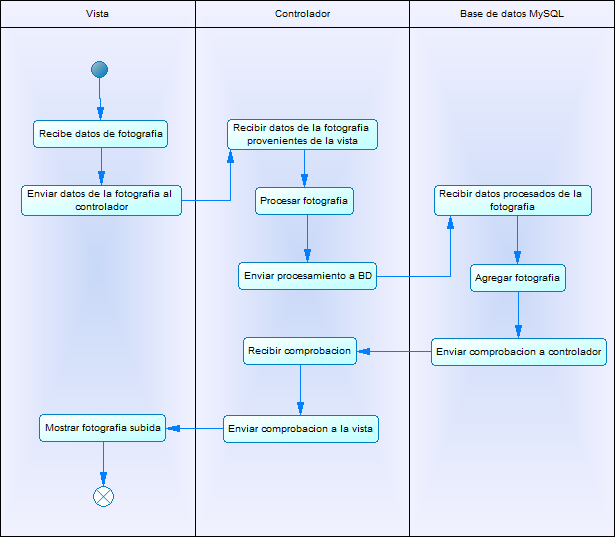
\includegraphics[width=15cm]{procesosCapa2SubirFoto.png}
}

En la figura 2-4 presenta el camino que tiene que seguir la información para cargar una foto al sistema de \textsl{BitPhoto}. Primero la vista recibe la información de la foto y la envía al controlador, éste es el encargado de procesar la información recibida por la vista para enviarla a la base de datos, que luego recibe la información y actualiza ls tablas con la información recibida y se vuelve a enviar al controlador que recibe una comprobación que se subió con éxito la fotografía y la envía a la vista para informar al usuario.

\newpage
\textbf{PROCESO HACER COMENTARIO.}

\figura{Capa 2 del Diagrama de Procesos, hacer comentario.}{
	\centering
	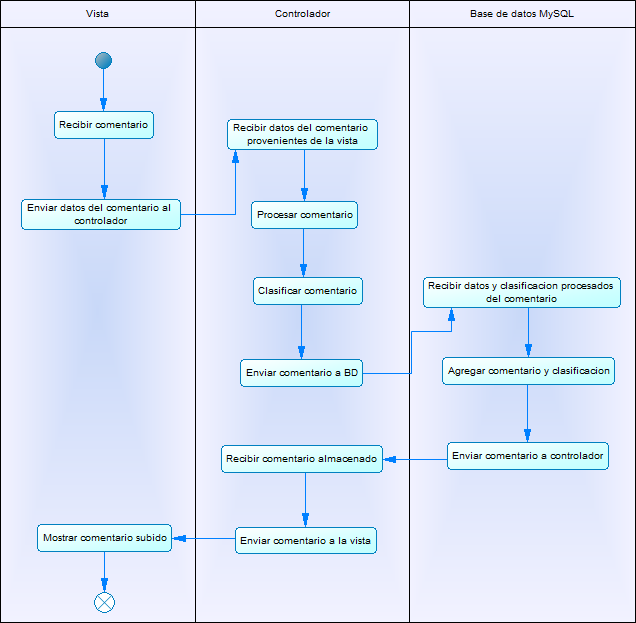
\includegraphics[width=15cm]{procesosCapa2Comentario.png}
}

En la figura 2-5, se muestra el proceso para hacer un comentario. Para iniciar el proceso de agregar un comentario al sistema se recibe el comentario en la vista y se envía la información al controlador, este procesa el comentario y también realiza el proceso de clasificarlo, al procesar todo lo del comentario se envía esta información a la base de datos que actualiza la información de esta y se envía nuevamente al controlador el comentario agregado al sistema y el controlador lo envía a la vista para mostrar el comentario agregado al sistema.

\newpage
\seccion{VISTA FÍSICA.}

En la vista física se presenta de qué manera se distribuyen los componentes de software en el medio físico del sistema. A continuación se presenta el diagrama de despliegue para identificar el hardware que utilizará el sistema y qué componentes tendrá. La idea de este diagrama es mostrar que mediante el despliegue y distribución de tecnologías en el hardware se pueden solucionar parte de los requisitos no funcionales.

\figura{Diagrama de despliegue de vista física.}{
	\centering
	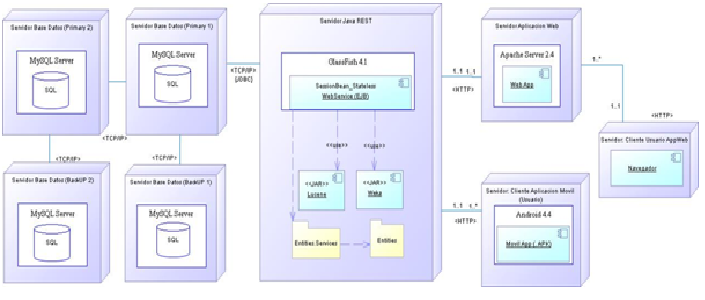
\includegraphics[width=15cm]{vistaFisica.png}
}

Para establecer una correlación con vista de desarrollo (ver sección 2.4), se muestran las siguientes asociaciones de cada parte de los diagramas correspondientes.

\begin{itemize}
\item Capa de Datos: Base de Datos – Packages (Entities).
\item Capa de Negocio: Servidor Java REST.
\item Capa de Presentación: Servidor Aplicación Web y Servidor Cliente Aplicación Movil, Servidor o PC usuario AppWeb.
\end{itemize}

Luego, para explicar el diagrama de la figura 2-6, se pueden desglozar sus partes mostrando las relaciones que se tienen y su función dentro del sistema.

\newpage
\begin{itemize}
\item \textbf{Base de Datos.}

\figura{Diagrama de despliegue: Base de Datos.}{
	\centering
	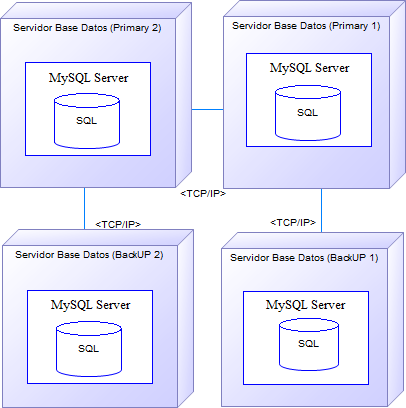
\includegraphics[width=10cm]{vistaFisicaBD.png}
}

La base de datos se encuentra distribuida en diferentes equipos (como se muestra en la figura 2-7), en este caso 2 servidores principales llamados \textsl{Primary 1} y \textsl{Primary 2}. Cada base de datos será respaldada en otros equipos en los servidores \textsl{BackUp 1} y \textsl{BackUp 2}. Estas bases de datos se comunicarán entre sí mediante protocolo TCP/IP. Esta distribución de base de datos permite mejorar la disponibilidad de los datos y en caso que los servidores principales se encuentren con problemas es posible acceder a los servidores de respaldo, además de mejorar la eficiencia dado de la lectura de las base de datos distribuidas mejora el tiempo de respuesta a las preguntas realizadas por el servidor del servicio REST.

\newpage
\item \textbf{Servicio Web.}

\figura{Diagrama de despliegue: Servidor Java REST.}{
	\centering
	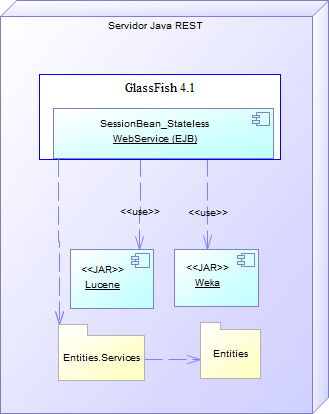
\includegraphics[width=10cm]{vistaFisicaRest.png}
}

Habrá un solo servidor destinado al servicio web (como se aprecia en la figura 2.8), el cual contendrá la lógica de la aplicación. Los EJBs se desplegarán en el servidor de aplicaciones \textsl{GlassFish} con el objetivo de ofrecer a los clientes (AppWeb y AppMovil) determinados servicios. En este servidor se encontrarán los componentes JAR de Weka y Lucene, además de los \textsl{packages Entities Services} y \textsl{Entities} que se utilizaran para la persistencia de datos. El servidor se comunicará con la base de datos mediante protocolo TCP/IP y con los clientes mediante el protocolo HTTP.

\newpage
\item \textbf{Aplicación Web.}

\figura{Diagrama de despliegue: Servidor Aplicación Web y Servidor Aplicación Móvil.}{
	\centering
	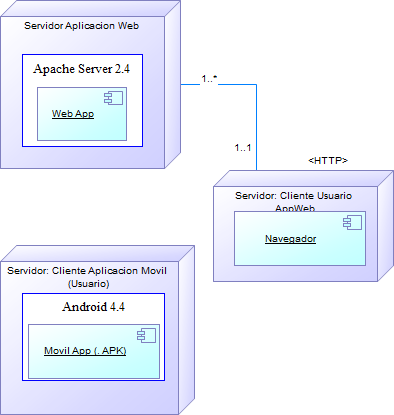
\includegraphics[width=10cm]{vistaFisicaUsuario.png}
}

La aplicación web se puede desplegar en un servidor distinto del servidor en el cual corre el servicio web (como lo muestra la figura 2-9). Este servidor contendría sólo a la aplicación web que consume el servicio ofrecido. Como se puede observar la aplicación web se encontrará desplegada en un servidor \textsl{apache}, el cual permitirá a los distintos usuarios acceder mediante sus navegadores web a la aplicación (Protocolo HTTP).

\item \textbf{Aplicación Móvil.}

Se despliega en el equipo del usuario, en este caso un dispositivo móvil, mediante un conjunto de paquetes de archivos de la aplicación (APK.) los cuales contienen las entidades encargadas de consumir el servicio web (Protocolo HTTP).
\end{itemize}

Cabe destacar que cada servidor puede ser replicado con el fin de mejorar la funcionalidad del sistema y la disponibilidad de este dependiendo de los requisitos no funcionales (como lo son la cantidad de llamados al sistema, la cantidad de usuarios concurrentes, entre otros). Una idea es agregar un servidor espejo al servidor web permitiendo mediante un cargador de peticiones (balanza) equilibrar la carga por parte de clientes.s


\seccion{VISTA DE DESARROLLO.}

En la vista de desarrollo se muestra mediante un diagrama de componentes la forma en la que se organizan los distintos componentes de software del sistema, que se caracterizan por su capacidad de desarrollo independiente del resto de los componentes. Para identificar de mejor manera los componentes, el sistema a desarrollar se divide en capas: capa de presentación, capa de negocio y capa de datos.

\figura{Diagrama de componentes de vista de desarrollo.}{
	\centering
	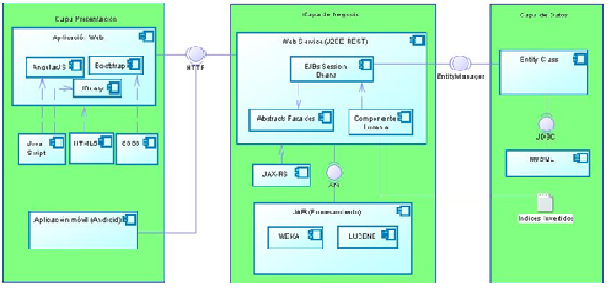
\includegraphics[width=16cm]{vistaDesarrollo.png}
}

\textbf{CAPA DE PRESENTACIÓN.}

En esta capa se encuentran los componentes que interactúan de manera directa con el usuario de la aplicación (ver figura2-11). Se observan los componentes \textsl{HTML5}, \textsl{JavaScript} y \textsl{CSS3} que permitirán la implementación de la interfaz del usuario, siendo estas tecnologías utilizadas por \textsl{AngularJS}, \textsl{JQuery} y \textsl{Bootstrap} que son los componentes dentro de la aplicación web necesarios para proveer páginas web dinámicas y de buen diseño. 

El framework \textsl{AngularJS} nos permitirá responder a eventos e implementar mediante funciones \textsl{JavaScript} las funcionalidades necesarias para conectarnos con el servicio web. Por otro lado está el componente de la aplicación móvil que se desarrollará utilizando la tecnología \textsl{Android}.  Ambas aplicaciones se conectarán con el servicio web en la capa de negocios mediante el protocolo HTTP. Cabe destacar que el servicio web ofrecerá métodos con los cuales los clientes web podrán acceder a la lógica de la aplicación.

\figura{Diagrama de componentes: Capa de Presentación.}{
	\centering
	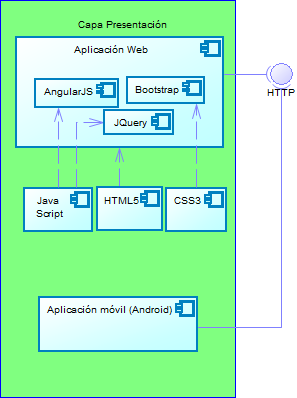
\includegraphics[width=9cm]{vistaDesarrolloCapaPresentacion.png}
}

\textbf{CAPA DE NEGOCIO.}

En esta capa se encuentra la lógica del negocio, representada mediante EJBs de tipo \textsl{Session Beans} (ver figura 2-12) los cuales se exponen gracias a la API JAX RS como servicios web tipo REST.  Los \textsl{Session Beans} se comunican con el componente de Lucene que permitirán realizar el buscador, mediante un índice invertido que se encuentra en la capa de Datos. Los \textsl{Session Beans} heredan de la clase \textsl{Abstract Facade} donde se define la interfaz de comunicación entre los EJBs y las Entidades de persistencia. Mediante el \textsl{Entity Manager} se logra que los EJBs persistan y obtengan información de la base de datos. \\

En resumen los \textsl{Session Beans} poseen las funcionalidades necesarias para lograr entregar al cliente web, servicios acordes a sus necesidades. Cabe destacar que los EJBs utilizarán los componentes de Weka y Lucene entregados como JARs, éstos se desarrollarán de manera independiente en primera instancia, permitiendo así, el trabajo modular por parte de los desarrolladores, para luego conectarlos con la lógica de la aplicación.\\

\figura{Diagrama de componentes: Capa de Negocio.}{
	\centering
	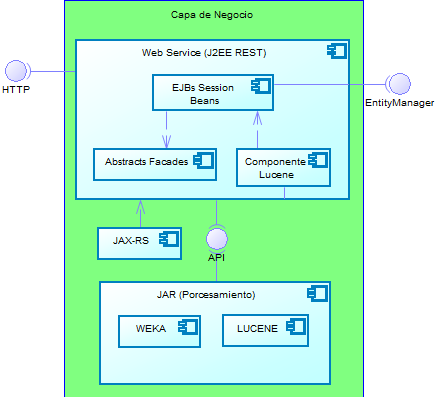
\includegraphics[width=12cm]{vistaDesarrolloCapaNegocio.png}
}

\textbf{CAPA DE DATOS.}

En esta capa se encuentran los componentes que permiten persistir la información necesaria para el funcionamiento del sistema, como lo es la base de datos propia de la aplicación y el fichero con los índices invertidos que utiliza Lucene (ver figura 2-13). La base de datos será implementada en el gestor de base de datos relacionales \textsl{MySQL community Edition}, que utiliza el servidor \textsl{MySQL sever} para permitir trabajar desde una entidad externa con la base de datos. 

La lógica de la aplicación implementada en JavaEE se conecta con la base de datos mediante el JDBC mapeando y generando \textsl{Entities} como un package, que son clases en java que representan las tablas que se encuentran en la base de datos. Como señalamos con anterioridad la capa lógica se comunica mediante el \textsl{Entity Manager} con los objetos de la base de datos. Permitiendo al sistema persistir e interactuar con los datos persistidos.

\figura{Diagrama de componentes: Capa de Datos.}{
	\centering
	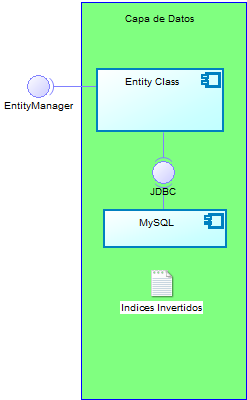
\includegraphics[width=6cm]{vistaDesarrolloCapaDatos.png}
}

\newpage
\seccion{ESCENARIOS.}

En los escenarios, se realiza la esquematización de la comunicación de las clases en la aplicación, para esto se utilizan los casos de usos más representativos de la aplicación, mostrados a continuación.

\subseccion{SUBIR FOTOGRAFÍA.}

\figura{Diagrama de Secuencia: Subiendo Fotografía.}{
	\centering
	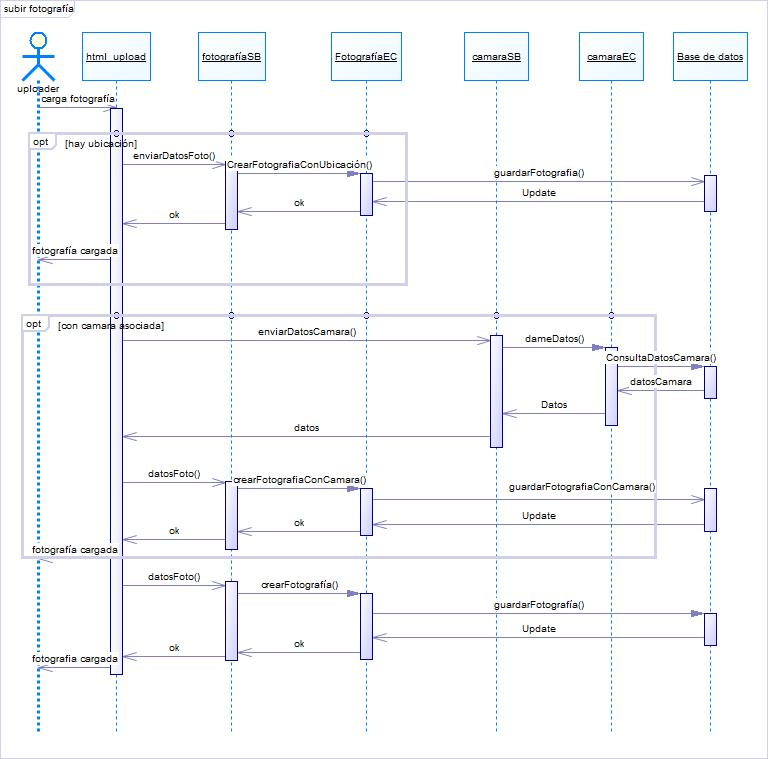
\includegraphics[width=15.8cm]{escenariosSubirFoto.jpg}
}

Para comenzar, se utiliza el caso de uso más representativo de la aplicación a desarrollar: Subiendo Fotografía. En este caso de uso se utilizan las clases \textsl{fotografíaSB}, \textsl{fotografíaEC}, \textsl{CamaraSB}, \textsl{CamaraEC}, además de la utilización de una vista llamada \textsl{html\_upload} y la base de datos como tal para realizar las consultas necesarias, tal como se aprecia en la figura 2-8.

Al iniciar se tiene un actor nombrado \textsl{Uploader}, que es el encargado de subir la fotografía, así este se posiciona en la vista \textsl{html\_upload}, la cual solicitará cargar una fotografía a elección por el actor. Luego la clase \textsl{FotografíaSB} recibe estos datos de la fotografía, para decidir que realizar. Pueden suceder tres casos que se detallan a continuación:

\begin{enumerate}
\item Si la fotografía es subida con una ubicación asociada, \textsl{fotografíaSB} recibe los datos de la fotografía cargada y envía estos datos a \textsl{fotografíaEC}, donde esta clase será la encargada de realizar la consulta para que así la base de datos cree la tupla con la nueva fotografía y actualice sus tablas.

\item Si la fotografía al momento de ser cargada tiene una cámara asociada, \textsl{fotografíaSB} se comunica con \textsl{CamaraSB} que es la encargada de recibir un identificador de una cámara, donde le solicita a la clase \textsl{CamaraEC} que le entregue los datos de la cámara pasándole a la vez el identificador de la cámara que necesita. Así \textsl{CamaraEC} es la encargada de consultar a la base de datos la información asociada a la cámara con el identificador correspondiente, de esta manera se los entrega a \textsl{CamaraSB} la cual le envía toda la información de los datos de la cámara a \textsl{FotografíaSB} que solicita a \textsl{Fotografía EC} que cree la tupla en la base de datos y la actualice.

\item Si no ocurre que la fotografía tiene una cámara o una ubicación asociada, se reciben los datos por \textsl{FotografíaSB}, que envía los datos correspondientes a \textsl{Fotografía EC}, que es la encargada de crear la tupla en la base de datos.
\end{enumerate}

\newpage
\subseccion{MAPA MUNDIAL.}

\figura{Diagrama de Secuencia: Visualizando mapa mundial de fotografías.}{
	\centering
	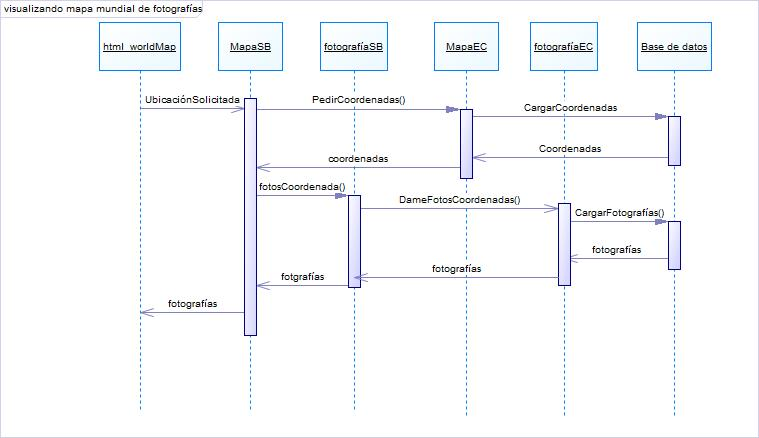
\includegraphics[width=17cm]{escenariosMapaMundial.jpg}
}

Para continuar con los escenarios, se muestra en la figura x-x un nuevo caso de uso denominado \textsl{Visualizando mapa mundial de fotografías}, el cual consiste en seleccionar una ubicación disponible en la vista \textsl{html\_worldMap}, para que así finalmente se visualicen las fotografías más populares en dicha ubicación.

Para este diagrama de secuencia se utilizan las clases \textsl{MapaSB}, \textsl{MapaEC}, \textsl{FotografíaSB}, \textsl{FotografíaEC} y una vista \textsl{html\_worldMap}, además de la correspondiente base de datos para las consultas pertinentes.

Para iniciar, se toma el supuesto que se ha seleccionado una ubicación dentro de la disponibilidad del mapa, donde \textsl{MapaSB} es la encargada de recibir tal ubicación para que envíe los datos a \textsl{MapaEC} con la finalidad de consultar las coordenadas correspondientes a dicha ubicación, de esta manera \textsl{MapaEC} recibe estas coordenadas y son enviadas a la clase \textsl{FotografíaSB} quien recibe las coordenadas para así comunicarse con \textsl{FotografíaEC} que realiza la consulta de las fotografías más populares en la ubicación con las coordenadas encontradas. Luego se entregan las fotografías y son visualizadas en la vista \textsl{html\_worldMap}.

\newpage
\subseccion{VER ÁLBUM.}

\figura{Diagrama de Secuencia: Ver álbum.}{
	\centering
	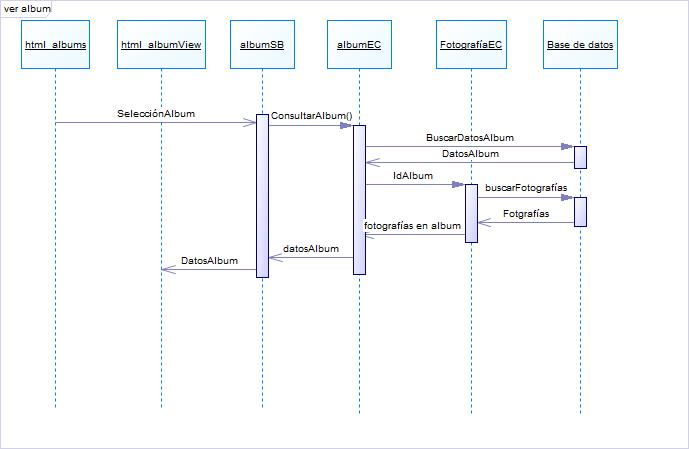
\includegraphics[width=17cm]{escenariosVerAlbum.jpg}
}

Para finalizar con los casos de usos más representativos, está el diagrama de secuencia correspondiente a \textsl{Viendo álbum}, donde se realizará una selección de álbumes disponibles, para que éste a su vez sea visualizado en la vista \textsl{html\_albumView}.

Para el diagrama de secuencia visualizado en la imagen anterior, se utilizan las clases \textsl{albumSB}, \textsl{albumEC}, \textsl{fotografíaSB}, \textsl{FotografíaEC}, las vistas \textsl{html\_albums}, \textsl{html\_albumView} y la correspondiente base de datos para las respectivas consultas necesarias.

Para iniciar el diagrama de secuencia, se toma el supuesto que el actor a seleccionado un álbum en la vista \textsl{html\_albums}, así \textsl{albumSB} captura el identificador del álbum seleccionado y solicita los datos del álbum a \textsl{albumEC}, donde ésta realiza la respectiva consulta para obtener el álbum asociado con dicho identificador, por consiguiente se necesitan las fotografías de dicho álbum, entonces \textsl{albumSB} solicita a \textsl{FotografíaSB} que le entregue las fotografías correspondientes, por lo cual esta última solicita a \textsl{FotografíaEC} que realice la consulta correspondiente a la base de datos para que así se entreguen las fotografías correspondiente y finalmente se visualice el álbum con sus fotografías correspondientes en la vista \textsl{html\_albumView}.


%-------------------------------------------------------------------------------------
\capitulo{MODELO 3-DIMENSIONAL SUNTONE.} 

\figura{Diagrama de Secuencia: Ver álbum.}{
	\centering
	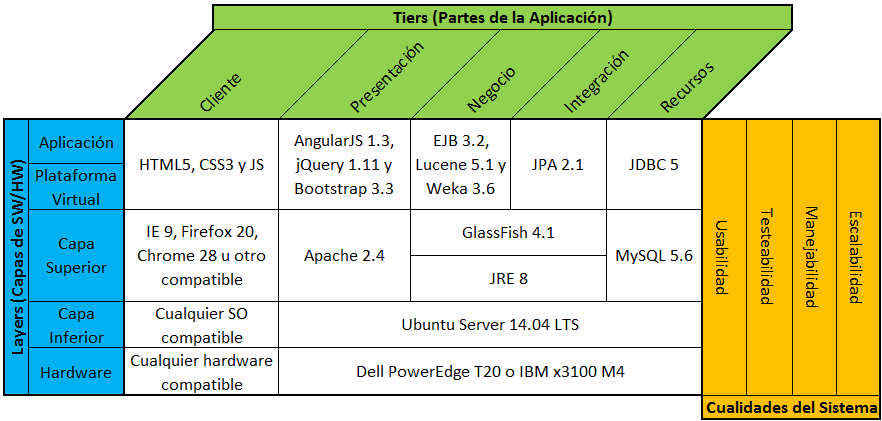
\includegraphics[width=16.5cm]{CuboTiersLayersCualidades.png}
}

En la figura 3-1 se ve representado el Cubo de \textsl{Tiers/Layers/Cualidades} con todas las tecnologías utilizadas en la aplicación a través de los \textsl{Layers} (capas de hardware y software) e intersectada con los \textsl{Tiers} (secciones lógicas de la aplicación).

Dentro de los \textsl{Layers} reperesentados en el cubo se destacan las versiones de cada tecnología de software utilizada. Dentro del \textsl{Layer} de Hardware destacamos algunos modelos de servidores capaces de sostener toda la plataforma de software antes descrita (Intel Xeon E3, 4GB RAM, 1TB HDD).

Para garantizar el funcionamiento correcto del sistema, se indica además las características deseables del sistema, las cuales se explican a continuación:

\begin{itemize}
\item \textbf{Escalabilidad}: la plataforma \textsl{BitPhoto} debe ser escalable en el sentido de poder ampliarse tanto en capacidad de cómputo (escalabilidad horizontal) al añadir servidores adicionales, y también debe ser ampliable en funcionalidad (escalabilidad vertical), facilitando el diseño modular y la incorporación de nuevos módulos funcionales.

\item \textbf{Manejabilidad}: los ejecutables de la plataforma \textsl{BitPhoto} deben ser fáciles de implementar en nuevos servidores.

\item \textbf{Testeabilidad}: la plataforma \textsl{BitPhoto} debe permitir y facilitar las pruebas unitarias e integradoras para permitir una validación rápida y expedita.

\item \textbf{Usabilidad}: la interfaz gráfica de \textsl{BitPhoto} debe permitir al usuario acceder rápidamente y sin esfuerzo a las funcionalidades que requiera, además de ser clara y no redundante.
\end{itemize}


%-------------------------------------------------------------------------------------
\capitulo{DEFINICIÓN DE FRAMEWORKS.}

Dentro de los distintos \textsl{FrameWorks} que se utilizarán para la implementación del sistema, se puede encontrar los de tipo Tecnológicos y Conceptuales.

\seccion{FRAMEWORKS TECNOLÓGICOS.}

\begin{itemize}

\item \textbf{AngularJS.}

Dentro de los diferentes \textsl{frameworks} que se aplican sobre la presentación de la aplicación, se destaca \textsl{AngularJS}, con un esquema ordenado de navegación para la aplicación y un patrón MVC claramente definido. Este \textsl{framework} plantea la creación de rutas, que determinan el archivo HTML de vista a cargar y su controlador propio asignado. Los controladores están programados en \textsl{JavaScript} y están fuertemente apoyados en la creación de objetos JS y del intercambio de éstos dentro de contextos (como \$scope).

\textsl{AngularJS} viene a solucionar el problema de mostrar los datos recibidos desde la capa de negocio. A través del protocolo REST, \textsl{AngularJS} puede recibir datos en formato JSON, procesarlos y desplegarlos de una manera agradable al usuario. Junto con ésto, las rutas de \textsl{AngularJS} se encargan de encapsular los elementos de la vista y desplegarlos al acceder via URL.
\end{itemize}

\seccion{FRAMEWORKS CONCEPTUALES.}

\begin{itemize}
\item \textbf{Modelo Vista Controlador (MVC).}

Dentro de \textsl{BitPhoto}, la arquitectura MVC se aplica dentro de la vista, al usuario del negocio (plataformas web y Android). En el caso de la plataforma web, el modelo es representado por los métodos que acceden a la capa de negocio, obteniendo objetos JSON a través de servicios de \textsl{AngularJS}. Los controladores, por su parte, son implementados directamente con \textsl{AngularJS}. La vista es elaborada en HTML5, CSS y JavaScript. En el caso de la plataforma \textsl{Android}, la arquitectura MVC se representa con módulos programados internamente en Java, usando el Paradigma Orientado a Objetos (POO).

La arquitectura MVC viene a ordenar todos los métodos de presentación del negocio, bajo una arquitectura bien consolidada y de alta interacción entre sus 3 módulos.

\item \textbf{Cliente-Servidor.}

El diseño Cliente-Servidor se aplica también a \textsl{BitPhoto}, ya que el núcleo de la aplicación está alojada en un servidor de aplicaciones (concentrando toda la lógica del negocio), mientras que los usuarios obtienen sus datos desde una aplicación cliente (en el caso de \textsl{Android}) o desde un navegador web (en caso de la aplicación web).

La arquitectura Cliente-Servidor permite que la aplicación servidora sea accedida mediante clientes remotos a través de redes de computación (como puede ser Internet). Además permite que los clientes no tengan que tener todos los métodos del negocio para poder usar la aplicación, reduciendo la carga de los módulos de aplicación para éstos.

\end{itemize}

%-------------------------------------------------------------------------------------
\capitulo{TECNOLOGÍAS A UTILIZAR.}

A continuación se describen las tecnologías a utilizar para la creación del proyecto, comenzando por la versión a utilizar, luego una breve descripción y también señalar problema que soluciona en nuestro sistema. Cabe destacar que se dividieron las herramientas y tecnologías en tres categorías asociadas al sistema, como lo es el \textsl{\textbf{Back-End}} asociada a la lógica del negocio o lógica de la aplicación, el\textsl{\textbf{Front-End}} que hace referencia a la parte del sistema que interactúa directamente con el usuario del sistema y de uso generalizado para el desarrollo del proyecto. Cabe destacar que las herramientas utilizadas se escogieron con el fin de lograr los requisitos planteados en la entrega anterior (Ingeniería de requerimientos).

\subseccion{BACK-END.}

\begin{itemize}
\item \textbf{JavaEE.}
	\begin{itemize}
	\item \textbf{Versión}: 7
	\item \textbf{Descripción}: es una plataforma de programación, es decir, un sistema que sirve como base para hacer funcionar distintos módulos de software con los que es compatible. Para desarrollar y ejecutar software, utiliza el lenguaje de programación Java. Su principal cualidad es facilitar el desarrollo de arquitecturas distribuidas y modulares, permitiendo distribuir en capas los distintos aspectos de la programación. Se constituye a partir de un conjunto de interfaces de programación de aplicaciones (API), el cual provee distintos protocolos, métodos y funcionalidades para desarrollar aplicaciones web.  La arquitectura Java EE, trabaja en un modelo de aplicaciones distribuidas en distintas capas, generalmente identificadas como capa de presentación, capa de datos y de negocios, siendo esta última en la cual interviene mayormente aprovechando las características que se mencionaron después.
	\item \textbf{Problema que soluciona}: por su estructura en capas permite modularizar el sistema a implementar, en diversas capas, como lo son la capa presentación, la de negocio, la de datos, entre otras que se pueden obtener de la subdivisión de las anteriores, permite que tengamos la capa de datos y lógica de negocio separada de la capa web o cliente.
	\end{itemize}

\item \textbf{API REST JavaEE 7.}
	\begin{itemize}
	\item \textbf{Versión}: 2.0
	\item \textbf{Descripción}: JAX-RS (\textsl{Java API for RESTful Web Services}) es una API del lenguaje de programación Java que proporciona soporte en la creación de servicios web de acuerdo con el estilo arquitectónico \textsl{Representational State Transfer (REST)}. JAX-RS usa anotaciones, introducidas en Java SE 5, para simplificar el desarrollo y despliegue de los clientes y puntos finales de los servicios web.
	\item \textbf{Problema que soluciona}: permite servir datos provenientes de la base de datos y métodos para poder trabajar con estos. Presenta EJB como servicios web, permitiendo así generar una arquitectura tipo cliente–servidor para el sistema a desarrollar, permitiendo a diversas aplicaciones comunicarse con el servidor para obtener información o persistir información.
	\end{itemize}
	
\item \textbf{Lucene.}
	\begin{itemize}
	\item \textbf{Versión}: 5.1.0
	\item \textbf{Descripción}: en una API de código abierto, que se agregará como biblioteca al proyecto en Java. Tiene como fin la recuperación de información, creada por Doug Cutting. Actualmente está apoyado por la fundación de software de \textsl{Apache} y se distribuye bajo la licencia \textsl{Apache Software License}.
	\item \textbf{Problema que soluciona}: en este caso se utilizarán sus características de indexado y búsqueda de texto para realizar el buscador de imágenes dentro de \textsl{BitPhoto}. Se basa en el concepto de documentos los cuales poseen determinados campos de texto, permitiendo así trabajar con diferentes formatos de texto.
	\end{itemize}
	
\item \textbf{MySQL Comunity Edition.}
	\begin{itemize}
	\item \textbf{Versión}:5.6.24
	\item \textbf{Descripción}: es un sistema que gestiona bases de datos tipo relacional y datos espaciales, con capacidad multihilo y multiusuario, desarrollado por \textsl{Sun Microsystems} (MySQL AB), aunque actualmente se desarrolla como software libre, además de poseer una versión comercial. \textsl{MySQL Comunity Edition} es un conjunto de programas que nos permiten almacenar, modificar y extraer información desde una base de datos, junto con proporcionar herramientas para añadir, borrar, modificar y analizar datos. También cabe destacar que proporciona métodos para mantener la integridad en los datos de la base de datos, controlando el acceso a usuarios, otorgando niveles de permisos para operar sobre la base de datos y recuperar información en caso de ser corrupta mediante una copia de seguridad. Todo lo señalado anteriormente está acompañado y representado mediante una interfaz cómoda y fácil de utilizar.
	\item \textbf{Problema que soluciona}: permite almacenar datos de la aplicación \textsl{BitPhoto}, información de los usuarios, álbumes, fotografías. En especial proporciona la capacidad de trabajar con datos geoespaciales, útil para referenciar una fotografía en el mapa.
	\end{itemize}
	
\item \textbf{Glassfish.}
	\begin{itemize}
	\item \textbf{Versión}: 4.1
	\item \textbf{Descripción}: es un servidor de aplicaciones desarrollado por \textsl{Sun Microsystems}, el cual implementa tecnologías definidas para JavaEE. Es gratuita y de código libre, pero también posee una versión comercial. Tiene como servidor base a \textsl{Sun Java System Application Server} de la corporación Oracle. El fin de utilizar \textsl{Glassfish} como servidor de aplicaciones es que permite proporcionar servicios a computadoras clientes, donde los clientes pueden acceder a los datos o conectarse con la parte lógica de la aplicación. Además es compatible con la plataforma JavaEE de esta forma se nos permitirá conectar con JavaEE RESTful.
	\item \textbf{Problema que soluciona}: permite presentar el servicio \textsl{Restful} para su consumo y presentar las aplicaciones clientes para consumir el servicio. Permite desplegar la aplicación de manera que pueda comunicarse mediante el local host con otras aplicaciones.
	\end{itemize}

\item \textbf{Java.}
	\begin{itemize}
	\item \textbf{Versión}: 8.45
	\item \textbf{Descripción}: Java es un lenguaje de programación de propósito general, concurrente, orientado a objetos que fue diseñado específicamente para tener tan pocas dependencias de implementación como fuera posible. Su intención es permitir que los desarrolladores de aplicaciones escriban el programa una vez y lo ejecuten en cualquier dispositivo, lo que quiere decir que el código que es ejecutado en una plataforma no tiene que ser recompilado para correr en otra.
	\item \textbf{Problema que soluciona}: lenguaje de programación que permite realizar toda o la mayoría del \textsl{Back-End}, cabe destacar que JavaEE utiliza como lenguaje nativo a Java, por lo cual toda la implementación del servició  RESTful se implementara utilizando Java.
	\end{itemize}
	
\item \textbf{WEKA.}
	\begin{itemize}
	\item \textbf{Versión}: 3.6.12
	\item \textbf{Descripción}: es una plataforma de software que se caracteriza por el aprendizaje automático y se utiliza frecuentemente en la minería de datos. Es una biblioteca escrita en Java y desarrollada por la Universidad de Waikato. Es un software distribuido bajo la licencia GNU GPL. Consiste en una colección de programas con algoritmos de aprendizaje que se encargan de procesar una serie de datos. Estos algoritmos se utilizan para entregar resultados luego de procesar los datos, mediante tareas de clasificación, regresión, asociación, entre otras.
	\item \textbf{Problema que soluciona}: con este conjunto de software se tiene como objetivo crear un analizador de sentimientos, para lo cual se entrenará un modelo con el fin de determinar los sentimientos de los comentarios que realizan los usuarios de \textsl{Bitphoto}, caracterizando estos como positivo, negativo o neutro.
	\end{itemize}
	
\item \textbf{NetBeans.}
	\begin{itemize}
	\item \textbf{Versión}: 8.0.2
	\item \textbf{Descripción}: es un entorno de desarrollo libre, creado principalmente para trabajar con el lenguaje Java. Posee una gran compatibilidad con diferentes tecnologías. Es un producto libre, aunque también existe una versión comercial. Para este proyecto se utilizará para realizar la integración entre las partes de nuestro sistema, conectar la base de datos con la lógica de la aplicación, así también con los módulos respectivos al buscador y clasificador, como también servir la aplicación creada.
	\item \textbf{Problema que soluciona}: permitirá integrar diversas tecnologías como lo son Gradle, JUnit, MySQL, GlassFish, JavaEE entre otras, para generar una solución íntegra y completa. Facilita el control de versiones mediante Git, y permite mediante sus APIs generar código de utilidad para el desarrollo del sistema RESTful y de la Aplicación Web.  
	\end{itemize}
\end{itemize}

\subseccion{FRONT-END.}

\begin{itemize}
\item \textbf{AngularJS.}
	\begin{itemize}
	\item \textbf{Versión}: 1.3.15 
	\item \textbf{Descripción}: es un \textsl{framework} de \textsl{JavaScript} de código abierto, mantenido con el apoyo de Google. Tiene como objetivo apoyar la creación de aplicaciones basadas en la capacidad del navegador con un modelo MVC, incluyendo así facilidades para el desarrollo y la prueba del código. El objetivo de utilizar esta herramienta está en desarrollar un esquema de aplicación web basado en rutas, potenciado por el uso de \textsl{JavaScript} y HTML5.
	\item \textbf{Problema que soluciona}: para el sistema a implementar facilita la integración de tecnologías web como lo son JS, CSS y HTML, permitiendo crear vitas más dinámicas y con mayor facilidad, y con menos sobrecarga del navegador.
	\end{itemize}
	
\item \textbf{Bootstrap.}
	\begin{itemize}
	\item \textbf{Versión}: 3.3.4 
	\item \textbf{Descripción}: es un \textsl{framework} de diseño web, libre y de código abierto, que contiene una colección de herramientas para la creación de sitios web y aplicaciones web. Contiene código predefinido HTML5 y plantillas CSS, para determinar la forma de los botones, textos, características en la navegación entre otras.
	\item \textbf{Problema que soluciona}: lo utilizaremos también para la creación de la interfaz web de \textsl{BitPhoto} con el fin de agilizar el desarrollo de la interfaz, al mismo tiempo que ésta queda con un diseño adaptativo y homogéneo.  
	\end{itemize}
	
\item \textbf{JQuery.}
	\begin{itemize}
	\item \textbf{Versión}: 1.11.3 
	\item \textbf{Descripción}: es una biblioteca de \textsl{JavaScript}, creada en un comienzo por John Resing. Esta biblioteca nos permite simplificar la manera de interactuar entre documentos HTML, manejar eventos, desarrollar animaciones, entre otras cosas. Todo esto complementado con la técnica AJAX para la creación de páginas web. Licencia MIT. JQuery.
	\item \textbf{Problema que soluciona}: otorgará funcionalidades basadas en \textsl{JavaScript} para la creación de \textsl{BitPhoto}, permitiendo lograr grandes resultados en menos tiempo y líneas de código.  
	\end{itemize}
	
\item \textbf{Android.}
	\begin{itemize}
	\item \textbf{Versión}: 4.4.2  
	\item \textbf{Descripción}: sistema Operativo basado en el Kernel de Linux, actualmente desarrollado por Google, y utilizado en dispositivos móviles de manera masiva. Se utilizara el \textsl{Target SDK} 19 para compatibilizar la aplicación con todos los dispositivos Android de versión 4.0 en adelante.
	\item \textbf{Problema que soluciona}: para este caso se desarrollará una aplicación compatible con este sistema operativo para que los usuarios de \textsl{BitPhoto} puedan hacer uso de éste a través de sus dispositivos móviles.
	\end{itemize}
	
\item \textbf{HTML.}
	\begin{itemize}
	\item \textbf{Versión}: 5  
	\item \textbf{Descripción}: lenguaje de marcado para la creación de páginas web. Es un lenguaje estándar que sirve de referencia para la elaboración de sitios web. Para nuestro caso permitirá definir una estructura básica para la interfaz de la aplicación y un código para la definición de contenido web como lo son textos, imágenes, videos, entre otros. Se utilizará el último estándar de este lenguaje que es HTML5.
	\item \textbf{Problema que soluciona}: será el lenguaje estándar web utilizado para realizar las vistas de la aplicación web. Permite trabajar junto con JS y CSS.
	\end{itemize}
	
\item \textbf{CSS.}
	\begin{itemize}
	\item \textbf{Versión}: 3  
	\item \textbf{Descripción}: hojas de estilo en cascada o CSS, lenguaje utilizado para la definición de plantillas web, para formatos HTML o XML. Permite estandarizar el diseño en la creación de aplicaciones web. La utilización de CSS 3, última versión de CSS. Permitirá estilizar uniformemente la apariencia de los elementos de la aplicación. 
	\item \textbf{Problema que soluciona}: proporciona una manera más simple de modificar el diseño de la vista, con nuevas funcionalidades CSS3 proporciona una vista con más posibilidades de diseño.
	\end{itemize}
	
\item \textbf{Javasript.}
	\begin{itemize}
	\item \textbf{Versión}: 1.8 
	\item \textbf{Descripción}: lenguaje de programación interpretado, esto quiere decir que se ejecuta del lado del navegador. Se caracteriza por ser orientado a objetos, basado en prototipos y se imperativo. Permite generar páginas web dinámicas. 
	\item \textbf{Problema que soluciona}: en este proyectos será de utilidad para la creación de páginas web dinámicas, destinadas  a responder a eventos y entregar información con un formato especificado.
	\end{itemize}
	
\item \textbf{Git (GitHub repositorio remoto).}
	\begin{itemize}
	\item \textbf{Versión}: 2.4.0  
	\item \textbf{Descripción}: es un software que permite controlar las versiones. Fue diseñado por Linus Torvalds, con el fin de controlar de manera eficiente y confiable las versiones de archivos de código fuente. 
	\item \textbf{Problema que soluciona}: el repositorio remoto a utilizar será proporcionado por \textsl{GitHub}, el que entrega espacio para desarrollar el proyecto, y conectar éste con los miembros del equipo de trabajo. 
	\end{itemize}
	
\item \textbf{Gradle.}
	\begin{itemize}
	\item \textbf{Versión}:2.3 
	\item \textbf{Descripción}: es una herramienta de automatización de proyecto, se basa en los principios de Apache Ant y Maven. Permite controlar y configurar el proyecto. Utiliza un grafo dirigido para determinar el orden de las tareas que se pueden ejecutar.  
	\item \textbf{Problema que soluciona}: para esta entrega se utilizará \textsl{Gradle} para compilar, desplegar, testear y controlar las diferentes dependencias del proyecto. 
	\end{itemize}
	
\item \textbf{JUnit.}
	\begin{itemize}
	\item \textbf{Versión}: 4.12 
	\item \textbf{Descripción}: es un conjunto de bibliotecas creadas para la programación, con el fin de realizar pruebas unitarias sobre diversos componentes de la aplicación, en especial las realizadas en Java. Permite ejecutar las clases creadas en Java, de manera controlada para evaluar el funcionamiento de los métodos implementados. Entonces en función de algún valor de entrada para la prueba se evalúa el valor retornado, si es el esperado o no. Controla las pruebas de regresión, para cuando el código sufra modificaciones corrobora si el nuevo código cumple con los requerimientos.
	\item \textbf{Problema que soluciona}: se utilizará para probar el programa java RESTful luego de cada modificación realizada en el código, comprobar que los métodos implementados retornan datos coherentes.
	\end{itemize}
\end{itemize}

%-------------------------------------------------------------------------------------
\capitulo{GESTIÓN DEL PROYECTO.}

\seccion{ORGANIZACIÓN DE REPOSITORIOS GIT.}
    
Para optimizar la creación de código, favorecer la correcta colaboración entre los integrantes y tener un versionamiento ordenado del código, se decide emplear a git como sistema de control de versiones, y usar GitHub como servidor remoto de git.\\

Cada miembro del grupo utiliza una cuenta de GitHub:

\begin{itemize}
	\item \textbf{Gerson Aguirre}: \textsl{https://github.com/GersonAguirre}
	\item \textbf{Max Chacón}: \textsl{https://github.com/nanochacon}
	\item \textbf{Daniel Gacitúa}: \textsl{https://github.com/GaciX}
	\item \textbf{Elías González}: \textsl{https://github.com/Elitos}
	\item \textbf{Nicolás Rozas}: \textsl{https://github.com/NicoRozas}
\end{itemize}

Se ha creado la organización “tbd2015” que aloja todos los repositorios del proyecto: \textsl{https://github.com/tbd2015}.\\

Dentro de la organización, se han creado diferentes repositorios para cada módulo del proyecto:

\begin{itemize}
	\item \textbf{InformesTBD}: Contiene los informes y presentaciones del proyecto. 
	\item \textbf{Prototipo}: Contiene el prototipo gráfico de la Aplicación Web.
	\item \textbf{BitPhoto}: Contiene el módulo principal del proyecto (en JavaEE).
	\item \textbf{BitPhoto-Mobile}: Contiene la aplicación para Android del proyecto.
	\item \textbf{BitPhoto-Search}: Contiene el motor de búsqueda (potenciado por Apache Lucene).
	\item \textbf{BitPhoto-Miner}: Contiene el módulo de análisis de sentimientos (potenciado por Weka).
\end{itemize}

Cada miembro del grupo tendrá acceso a todos los repositorios para fomentar la colaboración. Cabe destacar que con un sistema modular de repositorios dentro de la organización ordena de mejor manera los aportes de cada miembro y ayuda a evitar el entorpecimiento al hacer commits de forma concurrente.

\newpage

\seccion{COMUNICACIÓN, AVANCES Y BURNDOWN.}

En la segunda reunión de planificación realizada, se determinó que el segundo\textsl{sprint} duraría hasta el 16 de Mayo del 2015. Además se acordó las horas de trabajo diarias que se podían dedicar a la realización del proyecto, se estimó que cada integrante del grupo podría dedicar a lo máximo 1.5 hrs al dia para el proyecto. Luego se definieron las tareas para que estas se pudieran realizar en un tiempo cercano al de trabajo diario estimado y posteriormente se estimó el tiempo que se demoraría cada tarea en estar realizada.

Para la realización de la segunda entrega el grupo optó por varios canales de comunicación para manejar las relaciones entre los participantes, por lo tanto se determinaron distintas tecnologías para objetivos específicos, los canales usados para comunicarse entre el grupo fueron los siguientes:


\begin{itemize}
	\item Grupo \textbf{\textsl{WhatsApp}}, con el fin de conversar inmediatamente y de forma rápida temas relacionados con el proyecto, principalmente se utilizó para dudas cortas y compartir pequeñas opiniones del proyecto.
	\item Grupo \textbf{\textsl{Facebook}}, para registrar minutas, información relevante y noticias que afecten a todos los integrantes del grupo.
	\item Se creo una carpeta en \textbf{\textsl{Google Drive}}, para con el fin de compartir documentos referentes al informe, presentaciones, entre otras, correspondientes a la entrega de diseño arquitectural.  
	\item Se utilizó la aplicación \textbf{\textsl{Trello}} para organizar las partes que se debían realizar en la entrega, además esta aplicación permite organizar las partes del proyecto definiendo las tareas personalmente y los tiempos con los que fueron realizadas cada una de estas.
	\item Para controlar las versiones del informe y los prototipo de las vistas se utilizó la herramienta \textbf{\textsl{Git}} que permite controlar las versiones de estas dos partes del proyecto. Esta tecnología se utiliza para archivos de texto plano y para controlar las modificaciones que se le pueden realizar a éstos.
\end{itemize}

\newpage

A continuación se presentan las tareas definidas y los tiempos estimados.

\figura{Tareas 1-21}{
	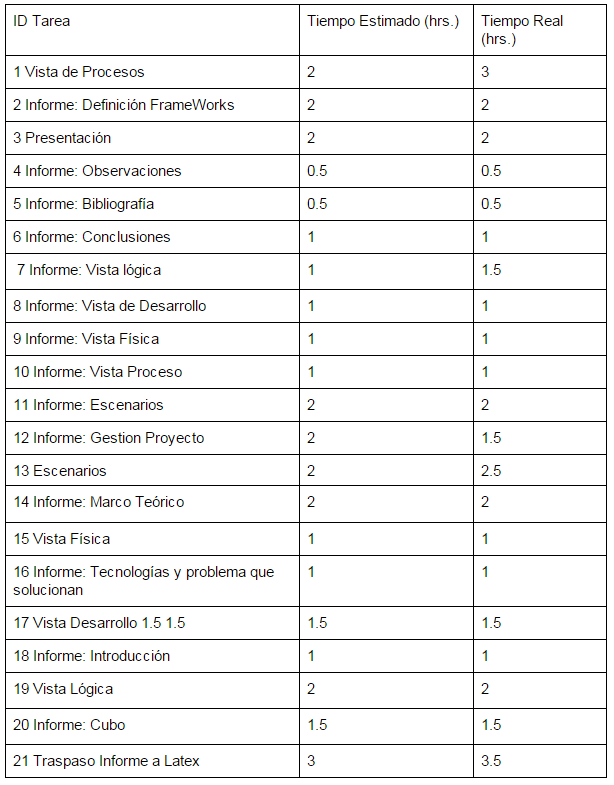
\includegraphics[width=15cm]{estimacionTareas1.png}
}


Ahora la cantidad de horas de trabajos estimadas son 31 hrs, Las horas de trabajo real fueron 33 hrs , notar que las horas reales trabajadas superaron las horas estimadas en 2 hrs aprox, esto quiere decir que las tareas se estimaron correctamente en su mayoría, ya que este margen de error fue relativamente bajo. Tiempo promedio por tarea fue de 1.48 hrs. Otros datos que se obtiene al analizar lo anterior son:

\begin{itemize}
	\item Estimación Trabajo Diario Grupo: 7.5 
	\item Horas Disponibles en Sprint por cada integrante: 37.5 
	\item Horas Disponibles en Sprint del Grupo: 187.5 
	\item Trabajo por dia promedio ideal 2.59 
\end{itemize}

Cabe señalar que si se trabajara de manera ideal, sobraría  tiempo equivalente a $187.5hrs - 31hrs = 156,5hrs$. 

A continuación se presentan los gráficos BurnDown y BurnUP con el fin de señalar la forma en que se trabajó a lo largo del Sprint.

\figura{Gráfico Burnup}{
	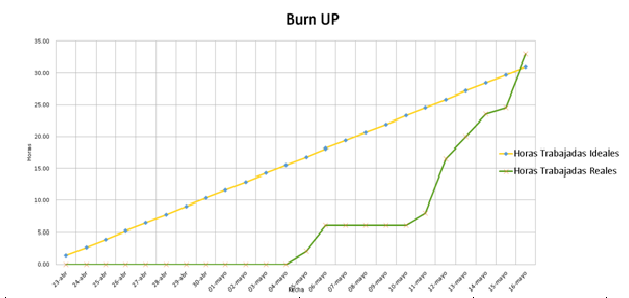
\includegraphics[width=15cm]{burnUp.png}
}

\newpage
\figura{Gráfico BurnDown}{
	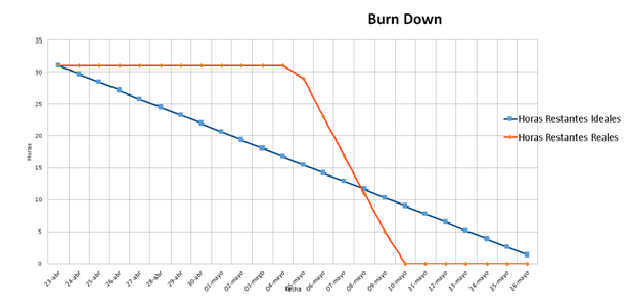
\includegraphics[width=15cm]{burnDown.png}
}

Como se aprecia en la imagen, se observa que en determinados periodos se trabajó una mayor cantidad, si bien alcanzamos a realizar la mitad del trabajo estimado a la fecha 8 de Mayo, se comenzó a trabajar en el proyecto varios días después de la planificación del \textsl{sprint}, por estos motivos se le solicitó al profesor mover la fecha de evaluación de la entrega de diseño arquitectural. Luego desde el 6 al 12 de mayo se comenzó a trabajar con gran rapidez, como se aprecia se terminó de ocupar las otras disponibles el 11 de mayo, el resto de los días si bien se trabajo, pero se trabajo tiempo superior al estimado.

Cabe destacar que para la próxima entrega se estimaron las tareas con \textsl{PokerPlaning} y se utilizará otra plataforma para realizar un análisis de datos, denominada \textsl{OllertApp}, la que facilitará el análisis de manera directa con lo realizado en \textsl{Trello}.

%-------------------------------------------------------------------------------------
\capitulo{OBSERVACIONES.}

Se añaden las observaciones realizadas al trabajo durante la 1º Presentación del Proyecto:

\tabla{Observación OBS1}{
	\begin{tabular}[c]{|p{4cm}|p{11cm}|}
		\hline
		Número Observación & OBS1\\ \hline
		Detalle Observación & Diagrama de Vista de Procesos mostrada en la presentación es en realidad Vista Física .\\ \hline
		Acción a Realizar & Diagrama mostrado se establece como Vista Física.\\ \hline
		Justificación & El diagrama mostrado permite representar de mejor manera la vista física que la de procesos.\\ \hline
		Página del Informe & 23\\ \hline
	\end{tabular}
}

\tabla{Observación OBS2}{
	\begin{tabular}[c]{|p{4cm}|p{11cm}|}
		\hline
		Número Observación & OBS2\\ \hline
		Detalle Observación & Eliminar servidor Android del diagrama de procesos mostrado (actualmente Vista Física).\\ \hline
		Acción a Realizar & Se elimina el servidor Android mostrado.\\ \hline
		Justificación & Servidor Android innecesario.\\ \hline
		Página del Informe & 23\\ \hline
	\end{tabular}
}

\tabla{Observación OBS3}{
	\begin{tabular}[c]{|p{4cm}|p{11cm}|}
		\hline
		Número Observación & OBS3\\ \hline
		Detalle Observación & Eliminar Managed Beans de los diagramas de secuencia de los Escenarios.\\ \hline
		Acción a Realizar & Se eliminan los Managed Beans de los diagramas de secuencia.\\ \hline
		Justificación & Innecesarios en el diagrama de secuencia, ya que no se utiliza Java Server Faces.\\ \hline
		Página del Informe & 31, 33 y 34\\ \hline
	\end{tabular}
}

\newpage

\tabla{Observación OBS4}{
	\begin{tabular}[c]{|p{4cm}|p{11cm}|}
		\hline
		Número Observación & OBS4\\ \hline
		Detalle Observación & Colocar Glassfish y JRE en la misma capa en diagrama 3-Dimensional SunTone.\\ \hline
		Acción a Realizar & Colocar Glassfish y JRE en la capa superior de los \textsl{Layers}.\\ \hline
		Justificación & Glassfish depende de JRE pero JRE no está por encima de Glassfish, por esto se colocan en la misma capa manteniendo JRE encima de Glassfish para representar la dependencia.\\ \hline
		Página del Informe & 35\\ \hline
	\end{tabular}
}

\tabla{Observación OBS5}{
	\begin{tabular}[c]{|p{4cm}|p{11cm}|}
		\hline
		Número Observación & OBS5\\ \hline
		Detalle Observación & Eliminar patrón DAO de la definición de \textsl{Frameworks}.\\ \hline
		Acción a Realizar & Eliminar DAO.\\ \hline
		Justificación & Patrón DAO no es un \textsl{Framework}, si bien viene implícito en JavaEE no se utiliza como tal.\\ \hline
		Página del Informe & 37\\ \hline
	\end{tabular}
}

%-------------------------------------------------------------------------------------
\capitulonn{CONCLUSIONES.}

Para la plataforma \textsl{BitPhoto}, es esencial diseñar correctamente el proyecto desde sus etapas más tempranas, es por eso que el Diseño Arquitectural es vital para el desarrollo y despliegue posterior de la aplicación.

El modelo 4+1 vistas y el Cubo 3D Suntone ayudan enormemente a llevar la visión de los arquitectos de software hacia los programadores, diseñadores y demás \textsl{stakeholders} de la aplicacion. En el contexto de la Ingeniería de Software resulta esencial comunicar correctamente la conceptualización de las ideas dentro del equipo de trabajo, para evitar inconsistencias en el producto final.

En esta entrega también se definen las tecnologías y sus versiones respectivas a utilizar dentro de la plataforma. Una clara definición del software y hardware que forman la plataforma condiciona la forma de trabajo, pero a la vez permite que los desarrolladores exploten de mejor manera los recursos tecnológicos disponibles.

Como siempre, la metodología ágil del proyecto implica constante comunicación entre los miembros del equipo desarrollador de \textsl{BitPhoto}. Llevando un control de las tareas desarrolladas se permite vigilar las cargas de trabajo.

Finalmente, se puede concluir que la plataforma \textsl{BitPhoto} pasó la etapa de Diseño Arquitectural, para iniciar posteriormente la etapa de Diseño Detallado. Los errores metodológicos a la hora de generar los esquemas y diagramas fueron debidamente corregidos.


%-------------------------------------------------------------------------------------

\capitulonn{BIBLIOGRAFÍA.}

[1] Philippe Kruchten. (Noviembre, 1995). En Planos Arquitectónicos: : El Modelo de “4+1” Vistas de la Arquitectura del Software(16). IEEE Software. 

Sitio Web: http://cic.puj.edu.co/wiki/lib/exe/fetch.php?media=materias:modelo4\_1.pdf

[2] SUNTONE ARCHITECTURE METHODOLOGY A 3-DIMENSIONAL APPROACH TO ARCHITECTURAL DESIGN. 11-Mayo-2015, de Sun MicroSystems 

Sitio web: http://rieck.dyndns.org/architecture/suntoneam\_wp\_5.24.pdf?version=1

[3] Chapter 2: Java Enterprise System Architecture. 11-Mayo-2015, de Sun Java Enterprise System 2004Q2 Technical Overview. 

Sitio web: https://docs.oracle.com/cd/E19263-01/817-5764/architecture.html

[4] Nicolás Tedeschi. ¿Qué es un Patrón de Diseño?. 11-Mayo-2015, de Microsoft 

Sitio web: https://msdn.microsoft.com/es-es/library/bb972240.aspx

[5] Juan Pavón Mestras. (2008-09). Estructura de las Aplicaciones Orientadas a Objetos El patrón Modelo-Vista-Controlador (MVC). 11-Mayo-2015, de Universidad Complutense Madrid 

Sitio web: https://www.fdi.ucm.es/profesor/jpavon/poo/2.14.MVC.pdf

[6] Libro J2EE Architecture \- B.V. Kumar, S. Sangeetha \& S.V. Subrahmanya [ISBN : 0070621632]

\end{document}
